%%%%%%%%%%%%%%%%%%%%%%%%%%%%%%%%%%%%%%%%%%%%%%%%%%%%%%%%%%%%%%%%%%%%%%%%
%
% Space Warps II: CFHTLS 
%
%%%%%%%%%%%%%%%%%%%%%%%%%%%%%%%%%%%%%%%%%%%%%%%%%%%%%%%%%%%%%%%%%%%%%%%%

\documentclass[useAMS,usenatbib,a4paper]{mn2e}
%% letterpaper
%% a4paper

\voffset=-0.6in

% Packages:
\input psfig.sty
\usepackage{xspace}
\usepackage{graphicx}
\usepackage{amssymb}
\usepackage{amsmath}
\usepackage{longtable}

% Macros:
% JOURNALS
\newcommand{\apj}{ApJ}
\newcommand{\apjl}{ApJL}
\newcommand{\apjs}{ApJS}
\newcommand{\mnras}{MNRAS}
\newcommand{\apss}{Ap \& SS}
\newcommand{\aap}{A\&A}
\newcommand{\aj}{AJ}
\newcommand{\prd}{Phys. Rev. D}
\newcommand{\nat}{Nature}
\newcommand{\araa}{ARA\&A}
\newcommand{\jgr}{J. Geophys. Res.}
\newcommand{\pasp}{PASP}

% MISC
\newcommand{\etal}{et~al.~}
\newcommand{\eg}{{\it e.g.\ }}
\newcommand{\ie}{{\it i.e.\ }}
\newcommand{\etc}{{\it etc.\ }}

\newcommand{\be}{\begin{equation}}
\newcommand{\ee}{\end{equation}}
\newcommand{\bea}{\begin{eqnarray}}
\newcommand{\eea}{\end{eqnarray}}


% CROSS-REFERENCING
\def\Sref#1{Section~\ref{#1}\xspace}
\def\Fref#1{Figure~\ref{#1}\xspace}
\def\Tref#1{Table~\ref{#1}\xspace}
\def\Eref#1{Equation~\ref{#1}\xspace}
\def\Aref#1{Appendix~\ref{#1}\xspace}

% UNITS
\newcommand{\kms}{\ifmmode  \,\rm km\,s^{-1} \else $\,\rm km\,s^{-1}  $ \fi }
\newcommand{\kpc}{\ifmmode  {\rm kpc}  \else ${\rm  kpc}$ \fi  }  
\newcommand{\pc}{\ifmmode  {\rm pc}  \else ${\rm pc}$ \fi  }  
\newcommand{\Msun}{\ifmmode {\rm M_{\odot}} \else ${\rm M_{\odot}}$ \fi} 
\newcommand{\Zsun}{\ifmmode {\rm Z_{\odot}} \else ${\rm Z_{\odot}}$ \fi} 
\newcommand{\yr}{\ifmmode yr^{-1} \else $yr^{-1}$ \fi} 
\newcommand{\hMsun}{\ifmmode h^{-1}\,\rm M_{\odot} \else $h^{-1}\,\rm M_{\odot}$ \fi}

% COSMOLOGY
\newcommand{\LCDM}{$\Lambda{\rm CDM}$}
\newcommand{\MS}{Millennium Simulation\xspace}

% LENSING
\def\zd{z_{\rm d}}
\def\zs{z_{\rm s}}
\def\Dd{D_{\rm d}}
\def\Ds{D_{\rm s}}
\def\Dt{D_{\Delta t}}
\def\Dds{D_{\rm ds}}
\def\Sigmacrit{\Sigma_{\rm crit}}
\def\REin{R_{\rm Ein}}
\def\MEin{M_{\rm Ein}}

% SOFTWARE/HARDWARE
\def\sw{{\small\sc Space\,Warps}\xspace}
\def\SW{{\sc Space\,Warps}\xspace}
\def\Talk{{\small\sc Talk}\xspace}
\def\Letters{{\small\sc Letters}\xspace}
\def\Letter{{\small\sc Letter}\xspace}
\def\Dashboard{{\small\sc Dashboard}\xspace}
\def\cfhtls{{\it CFHTLS}\xspace}
\def\python{{\sc python}\xspace}

% TABLES:
\newcommand\nodata{ ~$\cdots$~ }%

% PROBABILITY THEORY
\def\pr{{\rm Pr}}
\def\data{{\mathbf{d}}}
\def\datap{{\mathbf{d}^{\rm p}}}
\def\datai{d_i}
\def\datapi{d^{\rm p}_i}
\def\LENS{{\rm LENS}}
\def\saidLENS{{\rm ``LENS"}}
\def\NOT{{\rm NOT}}
\def\saidNOT{{\rm ``NOT"}}

% AGENT BUREAUCRACY
\def\effort{N_{\rm C}}
\def\experience{N_{\rm T}}
\def\skill{\langle I \rangle}
\def\contribution{$\sum_k \skill_k$}
\def\information{\delta I}

% COMMENTING
\usepackage[usenames]{color}
\newcommand{\question}[2]{\textcolor{red}{\bf Question from #1: #2}}
\newcommand{\flag}[2]{\textcolor{blue}{\bf Comment from #1: #2}}
\newcommand{\new}[1]{{\bf #1}}

% RESULTS
\def\Ncollaboration{XXX}

\def\oxford{Dept.\ of Physics, University of Oxford, Keble Road, Oxford, OX1 3RH, UK}
\def\oxfordeng{Dept.\ of Engineering Science, University of Oxford, Parks Road, Oxford, OX1 3PJ, UK}
\def\kipac{Kavli Institute for Particle Astrophysics and Cosmology, Stanford University, 452 Lomita Mall, Stanford, CA 94035, USA}
\def\ipmu{Kavli IPMU (WPI), University of Tokyo, 5-1-5 Kashiwanoha, Kashiwa 277-8583, Japan}
\def\zooniverse{Zooniverse, c/o Astrophysics Department, University of Oxford, Oxford OX1 3RH, UK}
\def\adler{Adler Planetarium, Chicago, IL, USA}
\def\lausanne{EPFL, Lausanne, Switzerland}
\def\zurich{Department of Physics, University of Zurich, Switzerland}
\def\paris{Institut d’Astrophysique de Paris, UMR7095 CNRS – Universit\'e Pierre et Marie Curie, 98bis bd Arago, 75014 Paris, France}
\def\icg{Institute of Cosmology and Gravitation, University of Portsmouth, Dennis Sciama Building, Portsmouth P01 3FX, UK}

\def\pjmemail{\tt pjm@slac.stanford.edu}
\def\amemail{\tt anupreeta.more@ipmu.jp}



%%%%%%%%%%%%%%%%%%%%%%%%%%%%%%%%%%%%%%%%%%%%%%%%%%%%%%%%%%%%%%%%%%%%%%%%

\title[\sw II]
{\SW: II. New lens candidates from the CFHTLS discovered
through citizen science}
    
\author[More et al.]{%
 % The \SW Collaboration includes:

% Principal Investigators (opt-out):
   \newauthor{%
    Anupreeta~More,$^{1}$\thanks{\amemail}
    Aprajita~Verma,$^{2}$
    Philip~J.~Marshall,$^{2,3}$
    Surhud~More,$^{1}$
    }
   \newauthor{%
    Elisabeth~Baeten,$^{4}$
    Julianne~Wilcox,$^{4}$
    Christine~Macmillan,$^{4}$
    Claude~Cornen,$^{4}$
   }
   \newauthor{%
    Amit~Kapadia,$^{5}$
    Michael~Parrish,$^{5}$
    Chris~Snyder,$^{5}$
    Christopher~P.~Davis,$^{3}$
    Raphael~Gavazzi,$^{6}$
    }
   \newauthor{%
    Chris~J.~Lintott,$^{2}$
    Robert~Simpson,$^{2}$
    David~Miller,$^{4}$
    Arfon~M.~Smith,$^{4}$
    Edward~Paget,$^{4}$
    }
   \newauthor{%
    Prasenjit~Saha,$^{7}$
    Rafael~K\:{u}ng,$^{7}$
    Thomas~E.~Collett,$^{8}$
    }
%
\medskip\\
$^1$\ipmu\\
$^2$\oxford\\
$^3$\kipac\\
$^4$\zooniverse\\
$^5$\adler\\
$^6$\paris\\
$^7$\zurich\\
$^8$\icg\\

}

%%%%%%%%%%%%%%%%%%%%%%%%%%%%%%%%%%%%%%%%%%%%%%%%%%%%%%%%%%%%%%%%%%%%%%%%

\begin{document}
             
\date{to be submitted to MNRAS}
\pagerange{\pageref{firstpage}--\pageref{lastpage}}\pubyear{2013}

\maketitle           

\label{firstpage}

%%%%%%%%%%%%%%%%%%%%%%%%%%%%%%%%%%%%%%%%%%%%%%%%%%%%%%%%%%%%%%%%%%%%%%%%

\begin{abstract} 

The CFHT Legacy Survey has been searched for strong lenses with
semi-automated algorithms both at galaxy and groups scales. With the aim
of improving these lens finding robots, we carry out a blind lens search
in the complete \cfhtls \textsc{wide} survey with \sw. We describe the training
sample used for both training the citizen scientists that participated
in \sw and calibrating their performance. We generate realistic looking
simulated samples of lenses both at galaxy and group-scales as part of
this training sample. We present 61 new strong gravitational lens
candidates discovered from the \sw-\cfhtls search out of which 40
candidates are promising. Furthermore, we compile a sample of false
positives which can be used for robot testing, first of its kind for the
lensing community. The simulated sample is also used to make a
comparison between human performance against the robots. We find that
the XX per cent of the known lens sample is recovered and the new lens
sample has XX completeness with respect to the simulated sample. We make
available the following data products: simulated sample, simulation code
and the false positives sample at XXX.

\end{abstract}

% Full list of options at http://www.journals.uchicago.edu/ApJ/instruct.key.html

\begin{keywords}
  gravitational lensing   --
  methods: statistical    --
  methods: citizen science
\end{keywords}

\setcounter{footnote}{1}

%%%%%%%%%%%%%%%%%%%%%%%%%%%%%%%%%%%%%%%%%%%%%%%%%%%%%%%%%%%%%%%%%%%%%%%%%%%%%%

\section{Introduction}
\label{sec:intro}

%{\it Describe various lens finding algorithms and the motivation for this particular project with \cfhtls. Already searched by robots: enables comparison of techniques. Lenses not yet found by robots, detectable by humans? }

The last few decades have seen a rise in the discoveries of strong
gravitational lenses owing to the plethora of interesting applications
they have in astrophysics and cosmology. Strong lenses are routinely
used to probe the dark matter distribution from galaxy (ref) to cluster
scales (ref), to  study distant young galaxies by using the lensing
magnification as a natural telescope (ref), to test the cosmological
model by constraining cosmological parameters such as the Hubble
constant (ref) and dark energy (ref) and many more. Even though strong
lenses are rare, since a foreground massive object needs to be
sufficiently aligned with a distant background source to produce
multiple images, systematic lens searches have led to discovery of over
500 lenses till date (XXX add mld url). 

Rarity of lenses implies searching for them is a painstaking task.
Efficient automated methods are thus imperative to finding a reasonably
complete and pure sample of strong lenses.   



Since the inception of the first citizen science project, Galaxy Zoo, to
classify galaxy morphologies \citep{Lintott2008}, several astronomy
and non-astronomy projects have been launched by the Zooniverse leading
to many interesting project. For example, PlanetHunters
has discovered XXX transiting exoplanets \citep{Schwamb2012},
Supernova XXX add ref and XXX add ref


In Paper I, we describe \sw, an online system that enables crowd-sourced
detection of gravitational lenses. In this paper (referred to as Paper
II), we describe our first lens search with \sw in the \cfhtls data.

This paper is organised as follows. In \Sref{sec:sw} we give a brief
overview of the \sw system, focusing on the aspects most relevant to the
interpretation of the results of this first lens search. In
\Sref{sec:data} we introduce the \cfhtls imaging data and the known lens
samples from the \cfhtls. In \Sref{sec:}, we explain the training sample
generated to aid the \sw users in the lens search. In
\Sref{sec:results}, we present the new lens candidates and our findings.
We discuss the implications of our results for future lens searches in
\Sref{sec:discuss} and draw conclusions in \Sref{sec:conclude}.

%%%%%%%%%%%%%%%%%%%%%%%%%%%%%%%%%%%%%%%%%%%%%%%%%%%%%%%%%%%%%%%%%%%%%%%%%%%%%%

\section{Data}
\label{sec:data}
\subsection{The CFHT Legacy Survey}
\label{sec:data:cfhtls}

The Canada-France-Hawaii Telescope Legacy Survey (CFHTLS) is a
photometric survey in five optical bands ($u^*g'r'i'z'$) carried out
with the wide-field imager MegaPrime which has a 1~deg$^2$ field-of-view
and a pixel size of 0.186\arcsec. The \cfhtls \textsc{WIDE} covers a total area
of 171~deg$^2$ on the sky and it consists of four fields W1, W2, W3 and
W4. The field W1 has the largest sky coverage of 63.65~deg$^2$. The
fields W2 and W4 have similar sky coverages of 20.32~deg$^2$ and
20.02~deg$^2$, respectively\footnote{These numbers are estimated from http://terapix.iap.fr/cplt/table\_syn\_T0006.html}.
The field W3 has a sky coverage of 42.87~deg$^2$ and is more than twice
as large as W2 and W4. 

The \cfhtls imaging is very homogeneous and has great image quality. Most of
the lensed arcs are much brighter in the $g$ band thus, deep imaging in
this band is desirable. The limiting magnitude is 25.47 for the $g$ band
which goes the deepest among all of the five bands. The mean seeing in
the $g$ band is 0.78\arcsec. The zero point to convert flux to AB
magnitude for all bands is 30. These characteristics make \cfhtls ideal
to do visual inspection for finding lenses.  We use the data from the
final T0007 release taken from the Terapix
website\footnote{{http://terapix.iap.fr/cplt/T0006-doc.pdf}}
for this work.

We note that the \cfhtls is a niche survey with a unique combination of
wide imaging with deep sensitivity. It is a precursor to the ongoing
wide imaging surveys such as the DES, KIDS and HSC and planned surveys
such as the LSST. Searching for lenses with \sw in the \cfhtls will
teach us important lessons and help prepare us for these larger imaging
surveys.


%%%%%%%%%%%%%%%%%%%%%%%%%%%%%%%%%%%%%%%%%%%%%%%%%%%%%%%%%%%%%%%%%%%%%%%%%%%%%%

\subsection{Image Presentation in \sw}
\label{sec:data:impres}
%{\it Preparation of data: divide survey into overlapping tiles. Presentation of images. Uniform scales, to build intuition and avoid rescales due to bright objects. Arcsinh stretch, to bring out low SB features. Approximately optimized, how? Examples of images.}

Our aim is to do a blind lens search over the entire \cfhtls
\textsc{wide}. We use the $g$, $r$ and $i$-band color imaging which are
most useful for visual identification of lenses (and provide access to
the $u$ and $z$ band imaging through dashboard with additional tools
XXX). 

We make color composite images using publically-available
code\footnote{The open source  color image composition code used in this
work is available from \texttt{http://github.com/drphilmarshall/HumVI}}
following the prescription of \citet{Lupton2004}. Specifically, we first
rescale the pixel values of each channel image into flux units, and
then apply an arcsinh stretch. The stretch parameters are chosen
using a small random sample of images, to ensure that the background
noise is just visible, and that the centres of bright, intermediate
resdhift galaxies are not saturated. The color scales are chosen to
maximize the contrast between faint extended objects. These parameters
are then fixed during the production of all the tiles, in order to
allow straightforward comparison between one image and another, and for
intuition to be built up about the appearance of stars and galaxies
across the survey.  

We extract contiguous cutouts of size 81.84\arcsec\ (440 pixels) with an
overlapping region of 10\arcsec (54 pixels) between the neighbouring
cutouts resulting into $\sim$ 430 000 cutouts for the entire \cfhtls
\textsc{wide}. The size of the individual cutout is determined by
optimising factors such as the typical angular scales of gravitational
lenses, the number of objects seen in a single cutout and the total
number of image cutouts in the survey. It is possible that a lens
candidate happens to be too close to the edge of a cutout, the overlap
between neighbouring cutout allows the inspector to get a clearer view
of the same candidate in at least one of the cutouts. We note that since
the images are shown randomly, an inspector may not necessarily come
across the neighbouring cutout unless the inspector classifies a large
number of images. This is not a problem since our user base is extremely
large and we receive multiple classifications of the same cutout. 

%%%%%%%%%%%%%%%%%%%%%%%%%%%%%%%%%%%%%%%%%%%%%%%%%%%%%%%%%%%%%%%%%%%%%%%%%%%%%%

\subsection{Existing \cfhtls lens samples}
\label{sec:data:kls}

The \cfhtls data has been searched for lenses using semi-automated algorithms,
primarily, in the $g$ band where the predominantly  faint blue  source
galaxies are bright compared to the predominantly red deflector galaxies.
Here, we briefly mention the lens samples which were known to the authors
prior to the lens search with \sw.

At galaxy-scales, we focus on two primary lens searches. The \rf
\citep{Gavazzi2014} was used for finding compact rings or arcs around centers
of isolated and massive early-type galaxies. By subtracting the PSF-matched
$i$-band images from the $g$-band images, the algorithm looks for excess flux
in the bluer $g$-band. An object detector measures the properties of these
residual blue features, and candidates meeting length-width ratio and
tangential alignment criteria are then visually inspected to form the final
sample. \citet{Gavazzi2014} first selected some 638,000 targets as either
photometrically-classified early type galaxies, or objects selected to have
red centers and blue outer parts, from the T06 CFHTLS data release catalogs. 
14370 were found to show detectable blue residuals, and 2524 were visually
inspected, having passed the automatic feature selection process. This led to
a sample of 42 good quality (\texttt{q\_flag} = 3) and 288 medium quality
(\texttt{q\_flag} = 2) lens candidates. In addition to this well defined
sample, \citet{Gavazzi2014} reported a further 71 serendipitously detected
lens candidates.  From this sample of ``\rf candidates,'' the SL2S team
found, during their follow-up campaign, 39 confirmed lenses (and 17 promising
candidates). We use this sample of 39 ``confirmed \rf lenses'' in our
completeness analysis.

The second galaxy-scale lens search was to find edge-on galaxy lenses in
the \cfhtls \citep{Sygnet2010} by selecting the galaxy's profile from the
output of {\sc Sextractor} in the $i$~band and with low inclination
angle. This sample has about 3 promising and a total of 18 lens
candidates.
 
On the other hand, the \af \citet{More2012} was used for
finding blue arc-like features in the complete \cfhtls data withouth any
pre-selection on the type of the lensing object. The search was carried
out in the g-band which is the most efficient wavelength to find typical
lensing galaxies. This sample, called the SARCS, has 55 promising and a
total of 127 lens candidates and consists of both galaxy and
groups/cluster scale lens candidates. Arc finding is better suited for
lensed images or arcs with larger image separations i.e. more massive
systems like groups and clusters. Thus, the SARCS sample has mostly
groups/cluster-scale lenses and a few galaxy-scale lenses.

For the purposes of transparency and to help a little with their training, 
the volunteers participating in \sw-\cfhtls lens search were made aware of
these known lens samples. Images containing the systems from the above samples
were labelled as ``Known Lens Candidates'' in the Talk forum, where volunteers
have the opportunity to discuss their findings with other volunteers and the
science team. 


%%%%%%%%%%%%%%%%%%%%%%%%%%%%%%%%%%%%%%%%%%%%%%%%%%%%%%%%%%%%%%%%%%%%%%%%%%%%%%

\section{Training sample: Simulated lenses}
\label{sec:ts}

{\it State the importance}

% % % % % % % % % % % % % % % % % % % % % % % % % % % % % % % % % % % % % % % 
\begin{figure*}
\begin{center}
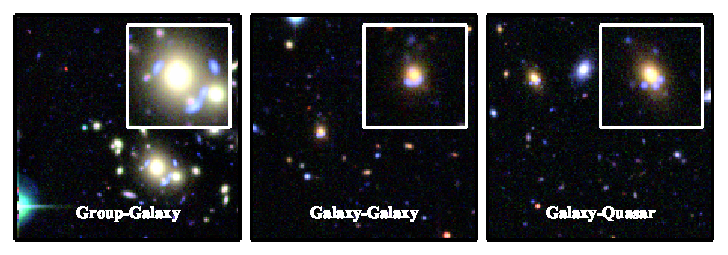
\includegraphics[scale=1.0]{sw-cfhtls-figs/sim_cgq.pdf}
\caption{ \label{fig:sim}
Examples of the three types of simulated lenses.
}
\end{center}
\end{figure*}


\subsection{Methodology}
\label{sec:simmethod}

We create two main types of simulated lens sample a) galaxy-scale lenses and b)
group or cluster-scale lenses. The galaxy-scale lenses are further divided into two
types based on the nature of the background sources, namely, galaxies and
quasars. Below, we describe how each type of the lens sample was generated.


\subsubsection{Galaxy-scale lenses} 
\label{sect:gallens}

The $N_{\rm src}$ behind a lens is then calculated by doing the
following integral, 

\be
\label{eqn:nsrc}
N_{\rm src} = N_{\rm src}(>L_s,z_s) \int_{z_l}^\infty \sigma_{\rm lens}(\sigma,z_l,z_s,q) D_s^2 (1+z_s)^2 \frac{\rm d\chi}{{\rm d}z_s}
{\rm d}z_s 
\ee

\be
\label{eqn:nlum}
 N_{\rm src}(>L_s,z_s)= \int_{L_{min}}^\infty \Phi(L_s,z_s) {\rm d}L_s
\ee

where $\Phi(L_s,z_s)$ is the source luminosity function per unit comoving
volume, $q$ is the projected axis ratio of the lens ellipticity, $\chi$ and
$D_s$ are the comoving and angular diameter distances to the source,

We use the elliptical galaxy (LRG) catalog from the \cfhtls XXX to select
all the foreground galaxies (e.g. $z<1$) that are potential lenses for the
simulated sample. We exclude all those galaxies whose positions match with the
lensing galaxies from the known \cfhtls~SL2S lens samples \cite{More2012}
within 2~arcsec (XXX check). 

First, we calculate the luminosity and velocity dispersion of each potential
lensing galaxy using the CFHT Megacam $g$ and $r$ band magnitudes along with the
photometric redshift ($z_l$) from the LRG catalog.  The Megacam magnitudes are
converted to SDSS magnitudes\footnote{
    http://www3.cadc-ccda.hia-iha.nrc-cnrc.gc.ca/megapipe/docs/filters.html} and
are further k-corrected to redshift $z=0.1$ \citep{Frei1994}. We assume that the
evolution of galaxy luminosities is similar to that determined by
\citep{Faber2007}, that is, a decline of $1.5$ in the $m_{r*}$ from redshift $z=1$
to $z=0$ (see Eq.~\ref{magstar}). 

\be
\frac{L}{L_{*}}=10.0^{-0.4~(m_{r \rm SDSS}-m_{r*})} 
\ee

where $m_{r*}$ is
\be
\label{magstar}
m_{r*}=-20.44+ 1.5~(z_{l}-0.1) \,.
\ee

We use the $L-\sigma$ relation from
\citep{Parker2005} to get the velocity dispersion as given in Eq.~\ref{magstar2}.

\be
\label{magstar2}
\sigma=142 \left(\frac{L}{L_{*}}\right)^{1/3} 
\ee

Next, in order to decide whether a galaxy is likely to act as a strong lens, we
calculate the lens cross-section ($\sigma_{\rm lens}$) and the number of sources
($N_{\rm src}$) that are in the background. Following \citep{Keeton2000a}, the lens
cross-section is calculated analytically for an isothermal model and is given by 

\be
\sigma_{\rm lens}=b_I^2 \, \int_0^{2\pi} 0.5 r^2(\theta) d\theta
\ee

where $b_I$ is 
\be
b_I = b_{\rm SIS} \epsilon_3/sin^{-1}(\epsilon_3) \,,
\ee

the eccentricity ($\epsilon_3$) is 
\be
\epsilon_3=(1-q_3^2)^{1/2}
\ee

and the projected axis ratio is given by
\be
q_k=\sqrt{q_3^2 {\rm sin}^2i_e+{\rm cos}^2i_e} \,.
\ee

In the above equations, $q_3$ is the 3d axis ratio of the ellipsoid and $i_e$ is
the inclination angle. Also, $b_{\rm SIS}= 4\pi
\frac{c^2}{\sigma^2}\frac{D_{s}}{D_{ls}D_l}$ and is referred to as the
Einstein radius where $D_s$,$D_l$ and $D_{ls}$ are angular diameter distances to
the source, the lens and between the lens and source, respectively.

%Comparing \citep{keeton00a} with \citep{kormann94} suggests that $b_I = sqrt(q)*b_{SIS}$ 

Next, if the foreground galaxy can act as a lens and has at least one source in the
background, then we determine a redshift ($z_s$) and $i$-band magnitude of the
background source(s). We assume two types of background sources namely, galaxies
and quasars. For each source, the redshift and magnitude are generated by drawing randomly from
the following redshift and luminosity distributions. For
galaxies, we assume the redshift distribution is 

\be
\label{eqn:ps}
p_s=\frac{\beta z_s^2 {\rm exp}({\frac{z_s}{z_0(m_{\rm lim})}})^\beta}{\Gamma(3/\beta)z_0^3(m_{\rm lim})}
\ee

where $\beta=3/2$ and $z_0(m_{\rm lim})=0.13m_{\rm lim} - 2.2$ and the
luminosity function is

\be
\label{eqn:ns}
n_s=\int^{m_{\rm lim}}_{-\infty} \frac{n_0 {\rm d}m}{\sqrt{10^{2a(m_1-m)}+10^{2b(m_1-m)}}}
\ee

with parameters $a=0.30$, $b=0.56$, $m_1=20$ and $n_0=3\times10^3~deg^{-2}$ as
given in \citep{Faure2009} and references therein. For quasars, we calculate
the luminosity function by following the prescription of \citep{Ogur2010} and
use k-corrections by \citep{Richards2006}. 

%alp=-0.5;
%kcorr=-2.5*(1 + alp)*log10(1+zz);
%Dlum=cc.Dlofz(zz)/p.hval;
%DM=5*log10(Dlum);
%Mabs=mag-kcorr-DM-25.0;
The luminosity function is expressed as
\be
\frac{{\rm d}\Phi}{{\rm d}M}=\frac{\Phi_{*}}{10^{0.4(\alpha+1)(M_{\rm abs}-M_{*})} + 10^{0.4(\beta+1)(M_{\rm abs}-M_{*})} }
\ee

where the normalization, $\phi_{*}=5.34\times10^{-6} h^3$ Mpc$^{-3}$ and break
magnitude, $M_*=-20.90 + 5 {\rm log} h - 2.5 {\rm log} f(z)$. The redshift
dependent factor in $M_*$ is given by

\be
f(z)=\frac{e^{\zeta z_s}(1+e^{\xi z_*})}{(\sqrt{e^{\xi z_s}}+\sqrt{e^{\xi z_*}})^2} \,.
\ee
We adopt the best-fit values $\zeta=2.98$, $\xi=4.05$, $z_{*}=1.60$
\citep{Oguri2010}. For the faint end slope, we use $\beta=-1.45$ whereas for
the bright end slope, we use $\alpha=-3.31$ when $z_s<3$ and $\alpha=-2.58$ at
higher redshifts, as prescribed by \citep{Oguri2010}. 
respectively. We note that when calculating $N_{\rm src}$, the source
number density is artificially boosted by a factor (see Table~\ref{tab:thresh})
to increase the occurrence of simulated lenses. This helps in creating a large
enough sample to carry out various performance tests.

Next, we determine properties of the background source for every lens. We follow
similar procedures for both background galaxies and quasars. For simplicity, we
simulate a single background source behind every lens. In order to select one
background source from the $N_{\rm src}$ per lens, we do ray-tracing for all of the
$N_{\rm src}$ sources with {\sc gravlens} \citep{Keeton2000} and choose sources that
satisfy criteria as given below. We determine fluxes of the lensed images
and the total magnification of each of the lensed source. We draw a random
source for which the flux of the second brightest lensed image and the total
magnification of all lensed images are above the thresholds given in
Table~\ref{tab:thresh}.

Since we want to produce realistic looking lens systems, we simulate lenses in
each of the five \cfhtls~filters. The colors of the background galaxies are drawn
randomly from the photometric CFHTLenS catalog
\citep{Hildebrandt2012,Erben2013}.  Similarly, we use a quasar catalog from the
SDSS Data Release 9 \citep{Paris2012} from which colors are drawn to simulate
quasar lenses. Next, we assume deVaucoleur's profile to account for the size
and shape of the galaxies. The ellipticity and the position angle are drawn
randomly between the range given in Table~\ref{tab:thresh}. The effective
radius of the galaxy is estimated from the Luminosity$-$size relation
\citep{Bernardi2003} given by 
\be
R_{\rm eff}= 10^{0.52} \frac{L_r^{2/3}}{{(1+z_s)}^2}
\ee
where $L_r=L_s/10^{10.2}$. On the other hand, quasars are assumed to follow a
Gaussian profile where the $\sigma$ is equated to that of the median seeing for
every filter. The median seeing values are taken from Table 4 of the official
Terapix T0007 release explanatory document \footnote{
    http://terapix.iap.fr/cplt/T0007/doc/T0007-doc.pdf}.  

Once all the parameters are determined for the lens and source models, {\sc
gravlens} is used to simulate lensed images.  After accounting for the shot
noise in the lensed images and convolving them with the median seeing in each of
the filters, the simulated image is added to the real \cfhtls~image centered
on the lensing galaxy. Note that we ensure that the lensed galaxies and
lensed quasars do not have the same lensing galaxy in the foreground. Similarly,
the lensing galaxies from the galaxy-scale lenses are distinct from the central
galaxies of groups-scale lenses which are described in the following section.


\begin{figure}
\begin{center}
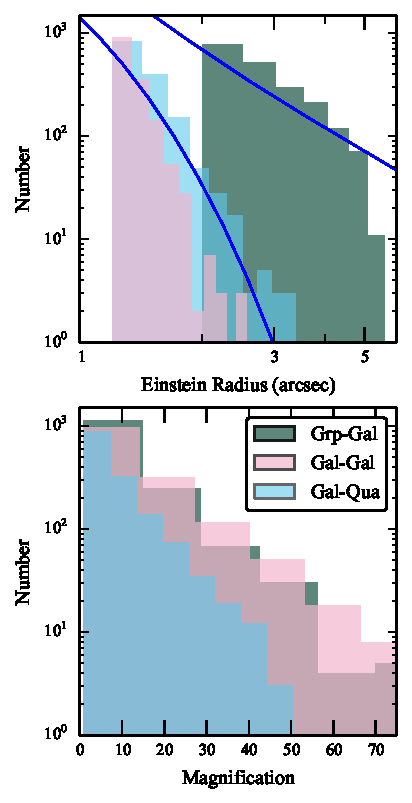
\includegraphics[scale=1.2]{sw-cfhtls-figs/distrib_remu.pdf}
\caption{ \label{fig:remudist}
Einstein radius distribution for all types of lenses. The dashed-dotted (blue)
curves show the theoretical prediction assuming an SIS model at galaxy-scales
and a total (NFW+Hernquist) model at groups-scales taken from \citep{More2012}.
}
\end{center}
\end{figure}


\begin{table}
\begin{center}
\caption{ \label{tab:thresh} 
Thresholds used in the selection of the simulated lenses. }
\begin{tabular}{l l l l l}
\hline
Name  &  \multicolumn{2}{c} {gal}  & \multicolumn{2}{c}{qso} \\ 
      & min  &  max  & min & max \\
\hline
\hline
Source Redshift  & 1.0 & 4.0  & 1.0  & 5.9 \\
Source Magnitude & 21.0 & 25.5 & 21.0 & 25.5 \\

boost factor & 100 (40$\dagger$)  &  & 1200 & \\

Second brightest image & 23  & & 23 & \\
Total magnification & 19 & & 20 & \\

Lens shear strength &  0.001 & 0.02 &  0.001 & 0.02 \\
Lens shear pa &  0 & 180 & 0 & 180  \\
Source ellipticity & 0.1 & 0.6 & & \\
Source PA & 0 & 180 & & \\
\hline
\end{tabular}
{ $\dagger$} -- corresponds to the factor used for Groups scale lenses. 
\end{center}
\end{table}
\subsubsection{Groups-scale lenses} 

At group or cluster-scales, the brightest group galaxy (BGG) at the center alone
does not cause strong lensing. We need to account for the extra convergence
arising from the dark matter component as well as satellite galaxies, at least,
in the inner regions which are typically responsible for the multiple lensed
images \citep{Oguri2005,Oguri2006}. Owing to the lack of an appropriate group
catalog for our purposes, we create a basic group catalog based on the
magnitudes and photometric redshifts available for the \cfhtls. We select all
galaxies with 10$^{10.8} M_\odot$ as the BGGs. We select the member galaxies
such that their photometric redshifts are within $\delta z = 0.01$ of the BGG
and within an aperture of $250$~Kpc. 

\begin{figure*}
\begin{center}
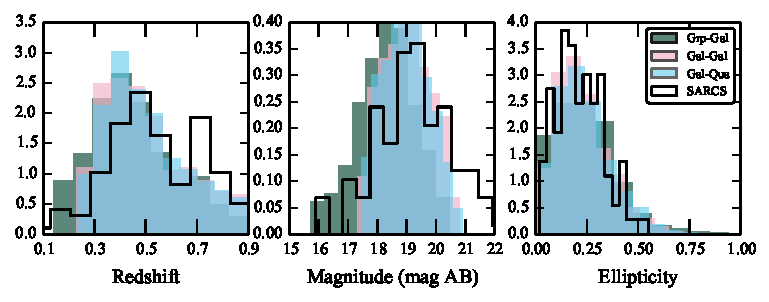
\includegraphics[scale=1.3]{sw-cfhtls-figs/lensprop.pdf}
\caption{ \label{fig:lensprop}
Distributions of properties of the lensing galaxies of the simulated
sample compared to the known lens sample SARCS XXXX check? 
}
\end{center}
\end{figure*}

We adopt an isothermal ellipsoid for the BGG and members whenever the
ellipticities are available else we use an isothermal sphere. On the other hand, we
adopt an NFW profile for the underlying dark matter halo. Assuming a constant
mass-to-light ratio of $3 \times 0.7$~h~$M_{*}/L_{*}$, we use the BGG luminosity
to estimate the stellar mass. The stellar mass$-$halo mass relation
\citep{behroozi13}, including random scatter, is then used to calculate the halo
mass for the lens. Given the halo mass, other key parameters such as the scale
radius ($r_s$) and the density at the scale radius ($\rho_s$) can be determined for an
NFW profile. 

As described in Section~\ref{sect:gallens}, we calculate the luminosity and
velocity dispersion for the BGG and each of the member galaxies. Next, we
calculate the lens cross-section for each potential lensing group. The
complexity in the lens models makes it analytically intractable to calculate the
size of the caustics\footnote{The lens mass distribution determines size and
shape of the caustics. Any source located within the caustics will form multiple
lensed images which is the criteria for strong lensing. To further
understand caustics, see XXX.}.  Hence, we use {\sc
gravlens} to determine the area covered by the caustics. We consider only
galaxies as our background source population since group or cluster-scale quasar
lenses are not expected to be found in the \cfhtls (check XXX).  Following the same
procedure as described in Section~\ref{sect:gallens}, we calculate the number of
galaxies expected to lie behind every potential lensing group (see
Eq.~\ref{eqn:nsrc}). As before, for each background galaxy within the lens cross-section, a
redshift and an $i$-band magnitude is determined by drawing galaxies randomly
from the respective distributions (see Eqs.~\ref{eqn:ps}-\ref{eqn:ns}). 

All those groups that are found to have no background galaxies within the
cross-sectional area are rejected and the rest are included as potential lenses.
As mentioned earlier, we artificially boost the total number of sources behind
every lens but ensure that (check XXX) the statistical properties such as the profile of the
image separation distribution are not affected (see \Fref{fig:remudist}). We
follow the same procedure and apply the same thresholds to determine properties
of the lensed galaxies for every lens as are described for galaxy-galaxy lenses
in the previous section. The simulated images are added to the real \cfhtls~images
with the BGGs as the center.

% % % % % % % % % % % % % % % % % % % % % % % % % % % % % % % % % % % % % % % 

\subsection{Simulated Lens Sample and Catalog Description}

In this section, we describe some of the properties of our simulated sample for
each of the three types of lens samples.

The \Fref{fig:remudist} shows Einstein radius distribution for the
galaxy-scale (dashed for background quasars and dotted for background galaxies)
and groups-scale simulated lenses. For comparison, we show the expected
distributions (blue dashed-dotted curves) for an SIS-like density profile at
galaxy-scales and an NFW+Hernquist profile at groups-scales. The 
theoretical curves are taken from \citep{More2012} wherein the models are
explained in detail. We note that the model we adopt at groups-scale also
includes SIS or SIE components for the group members unlike the theoretical
prediction. The theoretical curves have arbitrary normalizations.

We show the redshift and magnitude distributions of the lensing galaxies in the
left and right panels of \Fref{fig:lensprop}
respectively. Furthermore, we overplot the distributions of respective
properties of the SARCS lenses from \citep{More2012} for comparison with arbitrary
normalizations. We note qualitative similarities between the simulated and the
real lens samples.

Similarly, we show the ellipticity and the position angle of the simulated lens
galaxy population extracted from the T0007 release of the \cfhtls~catalogs in the
left and right panels of \Fref{fig:lensprop}, respectively. As before, the
dashed-dotted (blue) curves show the same distribution for the SARCS lens
population with arbitrary normalization \citep{More2012}.

%We show the source redshift and magnitude distributions for each of the three
%lens samples in the left and right panels of \Fref{fig:szmdist},
%respectively. The peak of the source redshift distribution both for the galaxies
%and quasars is known to be between $2<z<3$ from various lens samples (add
%references XXX). This consistent with our simulated sample as expected. The
%magnitude distribution of the simulated sample, on the other hand, is
%specifically tailored to the requirements of \sw.  The goal was to generate a
%lens sample that has a fair balance of both bright and faint lensed images since
%the training sample should neither be too easy nor too difficult for the citizen
%scientists.  

We produce catalogs with lens and source properties for each of the three types
of lenses. These catalogs are available XXX. The catalogs typically have lens
position, redshift, magnitudes, Einstein radius, ellipticity (whenever
available) and shear (for galaxy-scale lenses only). For the background
sources, we provide the offset from the lens center, redshift, magnitudes,
total magnification, number of lensed images. Additionally, ellipticity and
effective radius when the background sources are galaxies.

%magdiff=5*0.1;
%zdiffq=0.1;


%
%\begin{figure}
%\begin{center}
%\includegraphics[scale=0.95]{sw-cfhtls-figs/distrib_reff.eps}
%\caption{ \label{fig:reffdist}
%Distributions of magnification (left) and source effective radius in units of
%pixel (right).
%}
%\end{center}
%\end{figure}

% % % % % % % % % % % % % % % % % % % % % % % % % % % % % % % % % % % % % % % 

\section{Training sample: Duds and False positives}
\label{sec:dfp}

A good training sample consists of a representative set of objects that
one wants to find and another set of objects which appear to be from the
former set but are of different origin in reality and which one can
learn to discard efficiently. Indeed, we wanted to have a good training
sample for the \sw users so that they can correctly identify the true
lens candidates. Hence, in addition to the simulated lenses, we
added a sample of duds and false positives to the training sample. Duds
are images which have been visually inspected by experts and confirmed
to contain no lenses.  False positives are systems which look like
lenses but are not, for example, spiral galaxies, starforming galaxies,
chance alignments of features arranged in a lensing configuration and
stars. 

We selected a sample of 450 duds for the Stage I classification in \sw
and a sample of 500 false positives for the Stage II
inspection. The sample of false positives was selected from
the candidates which passed the Stage I of \sw. We note that this is the
first time, we have a systematically compiled sample of visually
inspected false positives by the \sw users and categorized by the
science team. Such a sample is tremendously helpful for training and
understanding performances of various lens finding algorithms
\citep{Chan2014}. {\bf TBA data products; make the duds and FP sample available}


\begin{figure}
\begin{center}
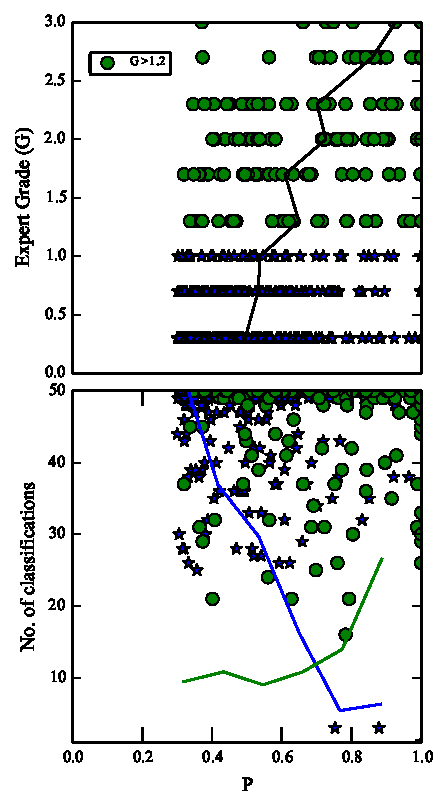
\includegraphics[scale=1.0]{sw-cfhtls-figs/poffl_expr_ncl.pdf}
\caption{ \label{fig:exp_pn} Comparison of the P(lens) with the expert
grades and number of classification for each subject.  }
\end{center}
\end{figure}

\begin{figure}
\begin{center}
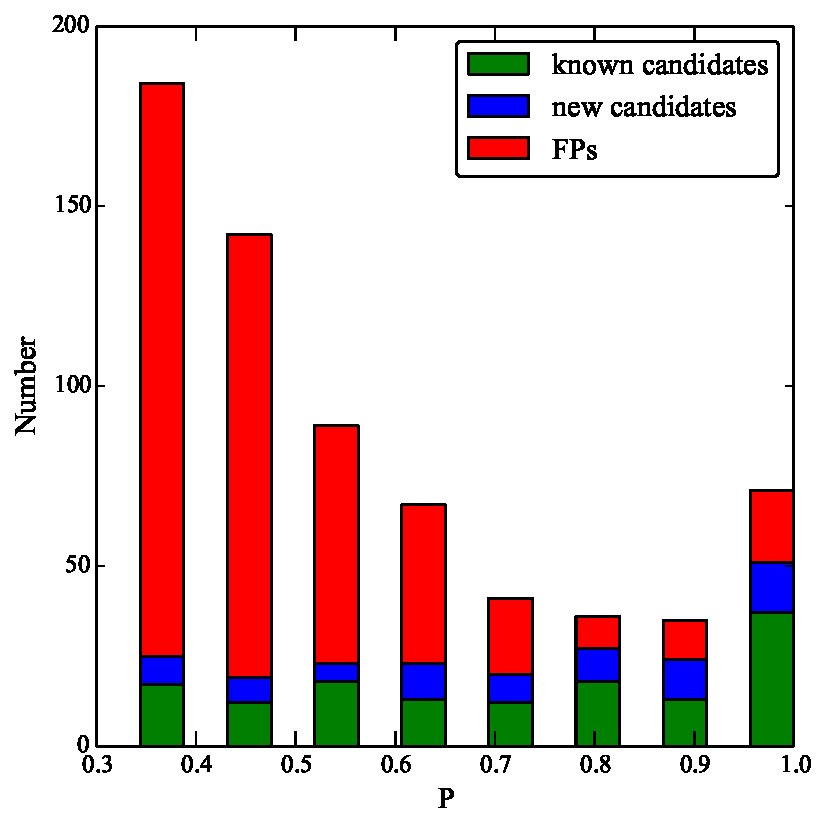
\includegraphics[scale=0.6]{sw-cfhtls-figs/cand_fp_P.pdf}
\caption{ \label{fig:stackP} Total number of detections of the known
candidates, new candidates and the FPs shown relatively for binned
values of P.
}
\end{center}
\end{figure}
%%%%%%%%%%%%%%%%%%%%%%%%%%%%%%%%%%%%%%%%%%%%%%%%%%%%%%%%%%%%%%%%%%%%%%%%%%%%%%

\section{Results}
\label{sec:results}

\subsection{\sw Lens Sample}

The \sw works as a single unified neural network which uses the method
of visual inspection to find gravitational lenses. The citizens are
shown images at two stages. At stage I, citizens focus on rapid
inspection and selection of lens candiates ranging from possible lenses
to almost certain lenses. At stage II, citizens carefully inspect the
candidates from stage I and select promising lens candidates only. The
science team consisting of lens experts then categorize and grade the
lens candidates further purifying the sample of lens candidates. In
Table~\ref{tab:stats}, we list the total number of detections of the
known lens candidates, known confirmed lenses and the new lens
candidates at both stages I and II. The known sample corresponds to the
combined Ring Finder and Arc Finder samples. We also show their
fractions with respect to the total number of lens candidates found at
these stages. We note that all the confirmed lenses found at stage I are
also recovered at stage II whereas a small fraction of the known lens
candidates are rejected at stage II. Also, the new lens candidates
increases the known lens candidates sample by over 50\%.

Below, we describe the steps taken after stage II for selecting the
final sample of lens candidates.

% % % % % % % % % % % % % % % % % % % % % % % % % % % % % % % % % % % % % % % 
\subsubsection{Selection of the \sw lens candidates}
\label{sec:results:stage1}
The images inspected in \sw are assigned probabilities (P) through the
\sw Analysis Pipeline (SWAP), built in the \sw system (see Paper I).
In an ideal situation, at the end of stage II, all images containing
lenses would have high P values and those without lenses will have low P
values. However, practically, a fraction of the real lenses will be
assigned low P value decreasing the completeness and a fraction of non-lenses
will be assigned high P value decreasing the purity. Our goal is to find
a P value which will result in acceptable levels of completeness and
purity of the final sample of lens candidates.  

As this is the first \sw lens search, we explore a large range in the P
value to understand the balance between the real lens candidates and
false positives. In \Fref{fig:exp_pn}, we plot the distribution of
false positives and real lens candidates categorized by the lens experts
as a function of their P value. As expected, the fraction of real lens
candidates is higher for higher P values and it decreases for lower P
values. We note that from P$\sim$0.7 onwards to lower P values, the fraction of
false positives starts to exceed the fraction of real lens candidates.
This could be a good threshold to choose to maximize the purity of the final
sample. However, we choose P$>$0.3 as our threshold to increase the
completeness of our sample. We achieve further purity by including the
grades of the lens experts.



\begin{table}
\begin{center}
\caption{ \label{tab:stats} 
Statistics of detections in \sw }
\begin{tabular}{l l l l l l l}
\hline
   &  \multicolumn{2}{c} {Stage I}  & \multicolumn{4}{c}{Stage II} \\ 
      & KC  &  KL  & KC & KL & NC & AC\\
\hline
\hline
Number  & 128 & 34 & 107  & 34  & 61 & 168\\
\%  & 29 & 58 & 25 & 58  & 12 & 34\\
P$_{\rm thresh}$ & 0.95 & 0.95 & 0.3 & 0.3 & 0.3 & 0.3\\

%% ####stage1
%% cand 128/436
%% conf  34/59
 
%% ####stage 2
%% sarcs conf 18/26
%% sarcs cand  55/106
%% RF conf 16/33
%% RF cand  52/330

\hline
\end{tabular}
\end{center}
{KC}-- Known lens candidates \\
{KL}-- Known confirmed lenses \\
{NC}-- New lens candidates  \\
{AC}-- All (known and new) lens candidates  \\
P$_{\rm thresh}$ -- systems with P above this threshold are selected \\
Note about \%: For KC and KL, fractions are with respect to the known
population whereas for NC and AC, fractions are with respect to the
total population of lens candidates. \\
\end{table}

% % % % % % % % % % % % % % % % % % % % % % % % % % % % % % % % % % % % % % % 

\subsubsection{New lens candidates from \sw}
\label{sec:results:disc}

All images with P$>$0.3, at the end of stage II, are inspected by three
lens experts (AM, AV, PJM) and are assigned integral grades from 0,1,2
or 3 which imply that the candidate is almost certainly not a lens,
possibly a lens, probably a lens and almost certainly a lens,
respectively. This process led to a final sample of 61 new lens
candidates with averaged grade $\ge$1.3 (see Table~\ref{tab:swcands})
and are shown in \Fref{fig:lc}. For this final sample, we give a \sw ID
and Name of the lens system, Ra, Dec, photometric redshift ($z_{phot}$),
$i$ band magnitude of the lensing galaxy, averaged grade from the lens
experts, zoo ID (identifier used in
TALK\footnote{http://talk.spacewarps.org/}, the discussion forum for
\sw), P value at stage II and a visual categorization of type of lensed
images and the lensing galaxy in the Comments column in
Table~\ref{tab:swcands}. Whenever available the lens properties are
taken from the \cfhtls photometric catalog \citep{Coupon2009} otherwise
the reported lens galaxy positions are measured visually. The visual
categorization of the lens type is only suggestive and the explanation
of the notations in the Comments column is given at the bottom of the
table.    

As the first lens search was a blind search with no preselection of
candidates using any algorithm, we expected to find various types of
lenses and this is indeed what we find. The final sample consists of
both galaxy and groups-scale lens candidates. There are detections of
elongated arcs and point-like quasar lensed images. Most of them are
brighter in bluer $g$ band but some candidates brighter in the redder
$i$ band are also found.


{\bf CHECK FOR STAGE 1 -- COMPLETENESS OF SIMS AND KNOWN LENSES
and P value comparison, what about the duplicate lenses near the borders
- stats on those?  check the detection plot of arc mag / Reinst and find out why some of
the bins have unexpected results}



\begin{figure*}
\begin{center}
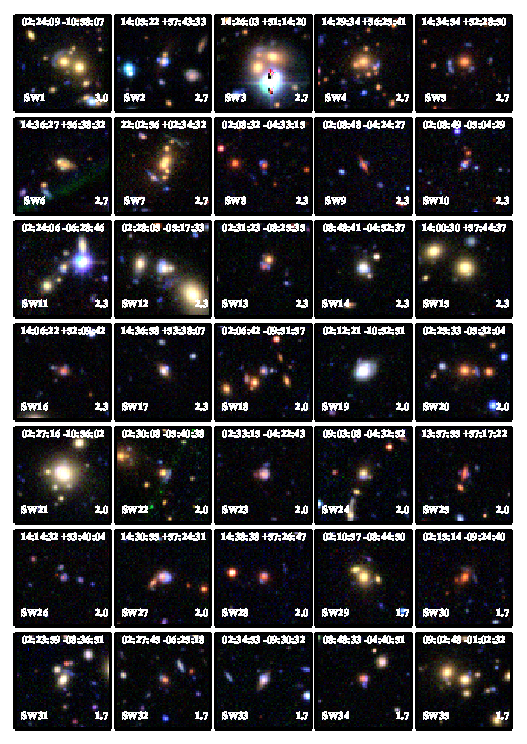
\includegraphics[scale=1.9]{sw-cfhtls-figs/lenscandfin.pdf}
\end{center}
\end{figure*}

\begin{figure*}
\begin{center}
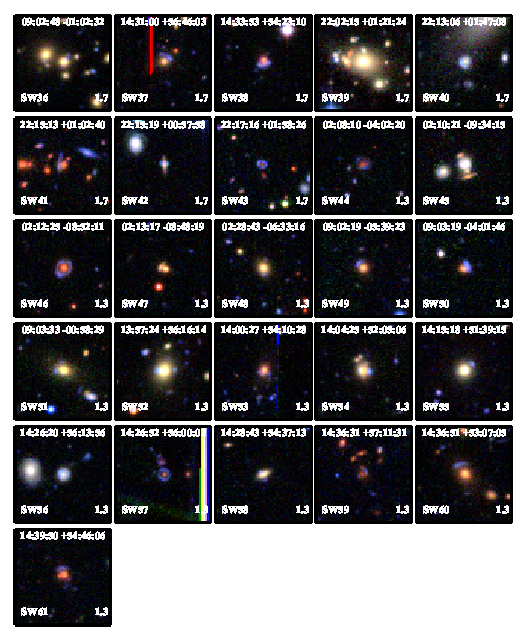
\includegraphics[scale=1.9]{sw-cfhtls-figs/lenscandfin_1.pdf}
\caption{ \label{fig:lc}
Sample of lens candidates with G$>=$1.3.
}
\end{center}
\end{figure*}
% % % % % % % % % % % % % % % % % % % % % % % % % % % % % % % % % % % % % % % 

\subsection{Measurements of lens and arc properties}
\label{sec:results:meas}

In the subsequent sections, we make comparison of various properties of
the lens candidates. Here, we describe how we measured those properties,
namely, the lens redshift, the Einstein radii and the total flux of the
arcs.

We use the publicly available redshifts for the lens galaxy from the
\cfhtls photometric catalogs \citep{Coupon2009}. The definition of the
Einstein radius is different in different cases. For the galaxy-scale
lenses in the simulated sample, we use the value of the input lens model
parameter for the $R_{\rm E}$. For groups-scale lenses, since the lens
model is multi-component, we need to determine the $R_{\rm E}$ from the
image positions. We use half of the averaged image separations of the
lensed image counterparts with minimum and maximum image separations.
For the \rf sample, the arcs are detected in the scaled difference image
between $g$ and $i$ bands where the lensing galaxy is subtracted
\citep[for details, see]{Gavazzi2014}. We use the peak position of the
lensed images measured by running {\sc sextractor} on this difference
image and identified visually. We calculate the image separation from
the lens center as an estimate of the $R_{\rm E}$. For the \af (SARCS)
sample, we use the same definition as above except that the peak
position is identified either by the \af or visually. For the \sw lens
sample, the same definition is used where the peak positions are
identified either with \af or {\sc sextractor}. 

The total flux of the arc is measured in the $g$ band. For the simulated
sample, we multiply the magnification of the second brightest image with
the source magnitude. For the \rf sample, we use the flux of the lensed
images measured by {\sc sextractor} from the scaled difference image,
that is, $g-\alpha i$ and convert it to the $g$ band flux using mean
colors of the foreground and background population. For the \af and the
\sw sample, we integrate the flux in the image pixels identified by \af
or {\sc sextractor}. 

% % % % % % % % % % % % % % % % % % % % % % % % % % % % % % % % % % % % % % % 

\subsection{Recovery of known \cfhtls lenses with \sw}
\label{sec:results:known}

We determine what fraction of the known sample of lenses are recovered by \sw. In
Table~\ref{tab:stats}, we show that $\sim$~25\%-30\% of the known
candidates and $\sim$~60\% of the known confirmed lenses are found at
stages I and II in \sw. The left and the middle panels of
\Fref{fig:compre} show the fraction of detections as a function of arc
magnitude and the Einstein radius of the lens systems. As expected, we
find that systems with brighter images and/or with larger Einstein radii
are detected more often in \sw. 

We find that most of the confirmed lenses and candidates that are missed by \sw
are systems with fainter arcs and smaller Einstein radii and they come
from the \rf sample. The main reason why \rf found such
candidates is because their team used lensing
galaxy-subtracted images to detect the presence of the lensed images
both during the automated object-finding phase and during the visual
inspection and classification of their candidates. This approach
naturally improves the detection efficiency at smaller Einstein radii
and for fainter systems. The \sw volunteers were not shown any
galaxy-subtracted images. However, in light of the improved detection
efficiency, this might be a better strategy to adopt for future lens
searches at galaxy-scales with \sw. In the Discussion \Sref{sec:fn}, we
further explore and discuss why the confirmed lenses may have been
missed in \sw. 

\begin{figure*}
\begin{center}
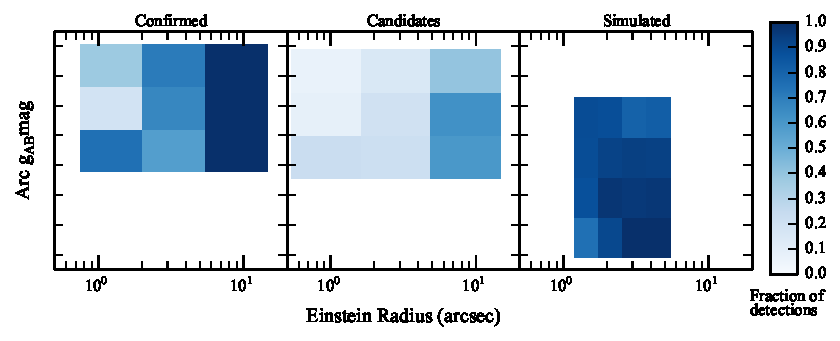
\includegraphics[scale=1.0]{sw-cfhtls-figs/comp_reinst_mag.pdf}
\caption{ \label{fig:compre} Fraction of lens candidates detected by \sw
as a function of the arc magnitude ($g$ band) and the Einstein radius for
three lens samples, namely, simulated lenses, known confirmed lenses and
the lens candidates sample. }
\end{center}
\end{figure*}


% % % % % % % % % % % % % % % % % % % % % % % % % % % % % % % % % % % % % % % 
\subsection{Image separation distribution}
\label{sec:results:isd}

The distribution of image separations (i.e. twice the Einstein radius)
can be used to probe the average density profile of the lens population
\citep{Oguri2006,More2012}.  However, the lens sample found
by the Arc Finder may have incompleteness as a function of the image
separation. Thus, the lack of understanding of the selection function of
the lens sample may affect the constraints on the density profile.  A
blind lens search done by visual inspection alone e.g. by \sw may find
lenses missed by the Arc Finder search and thereby, improve
completeness. Furthermore, the completeness of the lens sample found by \sw is
characterised with the help of the simulated sample. For example, in the
right most panel of \Fref{fig:compre}, we plot the completeness of the
simulated sample found at stage I of \sw as a function of the arc
magnitude and Einstein radius. We find that the sample is more than 80\%
complete between image separations 2"-10". 

In \Fref{fig:isd}, we plot theoretical curves for the image
separationd distribution corresponding to three density profiles,
namely, isothermal sphere (IS), NFW \citep{Navarro1997} and Total profile which has
NFW and Hernquist profiles combined with an adiabatically contracting model for
dark matter component \citep{Gnedin2004} taken from \citet{More2012}.
 


%%%%%%%%%%%%%%%%%%%%%%%%%%%%%%%%%%%%%%%%%%%%%%%%%%%%%%%%%%%%%%%%%%%%%%%%%%%%%%

\section{Discussion}
\label{sec:discuss}

Finding gravitational lenses is a difficult and complex task. No one
method is perfect. Each method has some advantages over the other. It
may be the case that a single method may not be the best means for
optimising completeness and purity. Visual inspection will likely be
required for pruning candidates at some stage of lens candidate
selection even in the future. Therefore, we would like to understand how
best we should combine the strengths of robots and humans to optimize
the lens finding method. 
  
In this section, we attempt to understand and compare the lens
(candidates) that are found by the lens finding robots and missed by humans
and vice versa.


\subsection{False negatives: known lenses missed by \sw}
\label{sec:fn}
Like any lens finding method, the \sw system can fail to detect
certain kinds of lenses. We explore and discuss why some of the known
confirmed lenses may have been missed. About 40\% of the known confirmed sample of
lenses are missed (see \Tref{tab:stats}). And, XXXX

Among the confirmed lenses from the \rf, about 50\% are missed. Out of
the missed sample of 18 lenses, about half of them are visually
difficult to detect and the other half seem to show faint blue smudges
around galaxies which should have been easier to identify.  {\bf Let us
compare the two samples to see if there are any obvious differences.
only 2 out of this sample of 18 were detected at stage I (reached high P
even with fewer classifications) and missed at stage II (P value was low
even after recieving very many classifications). The rest of the 16
lenses were rejected right at stage I XXX}

If we consider the \af lenses, only 6 out of the 26 ($\sim$23\%) were
missed by \sw. One of those 6 lenses was detected at stage I but failed
to get high enough P value at stage II even after receiving a total of
50 classifications (set as the upper limit). The rest of the 5 lenses
are already rejected at stage I. Upon visual inspection of these 5
systems, they appear to be difficult to identify as lenses because
either the lensed images are faint, have low curvature, are close to the
edge and/or are not visible due to proximity to an extremely bright
galaxy ({\bf show some examples XXX}). 


\begin{figure}
\begin{center}
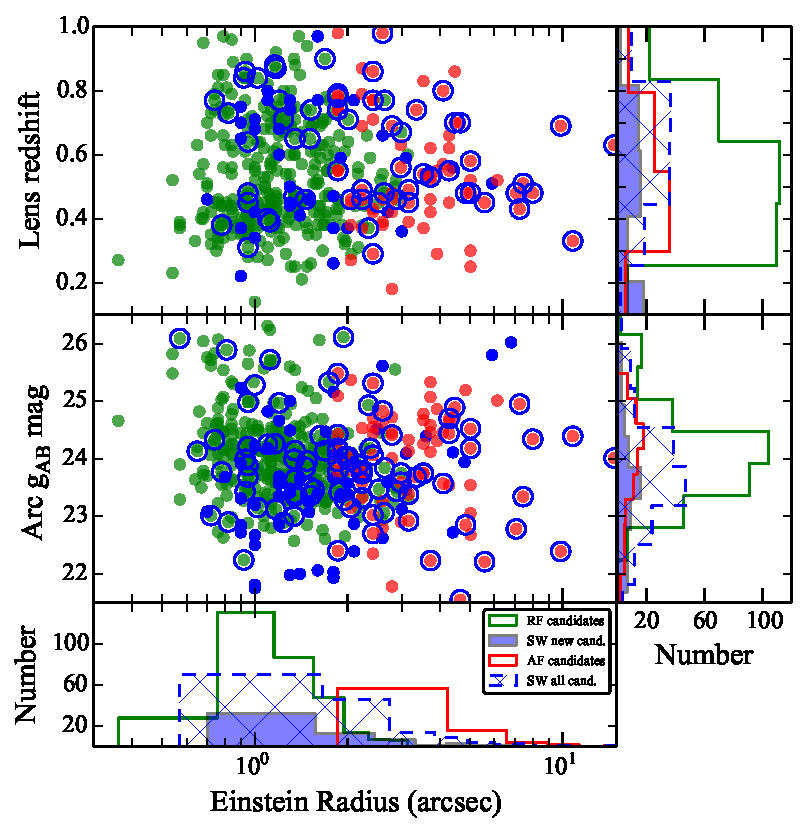
\includegraphics[scale=0.65]{sw-cfhtls-figs/zl_mg_re.pdf}
\caption{ \label{fig:zlre}
Comparison of the lens redshift and of the arc magnitude with the
Einstein radius for all of the three lens samples, namely, from the \rf (green dots),
\sw (all candidates black circles and new candidates only in blue dots)
and \af (red dots). }
\end{center}
\end{figure}

\begin{figure*}
\begin{center}
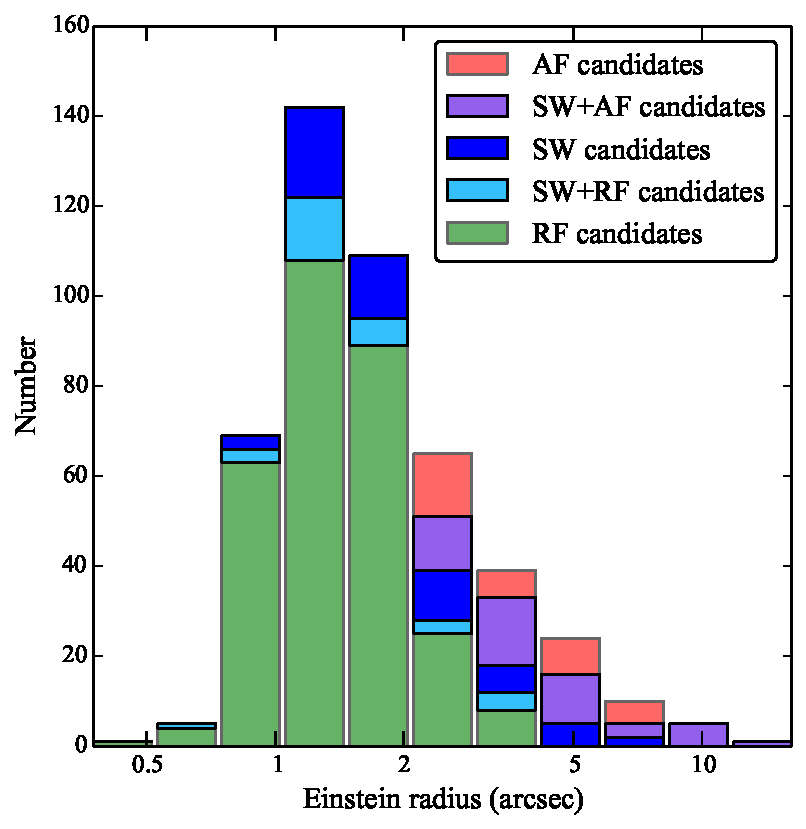
\includegraphics[scale=0.5]{sw-cfhtls-figs/stacked_lenscand_rein.pdf}
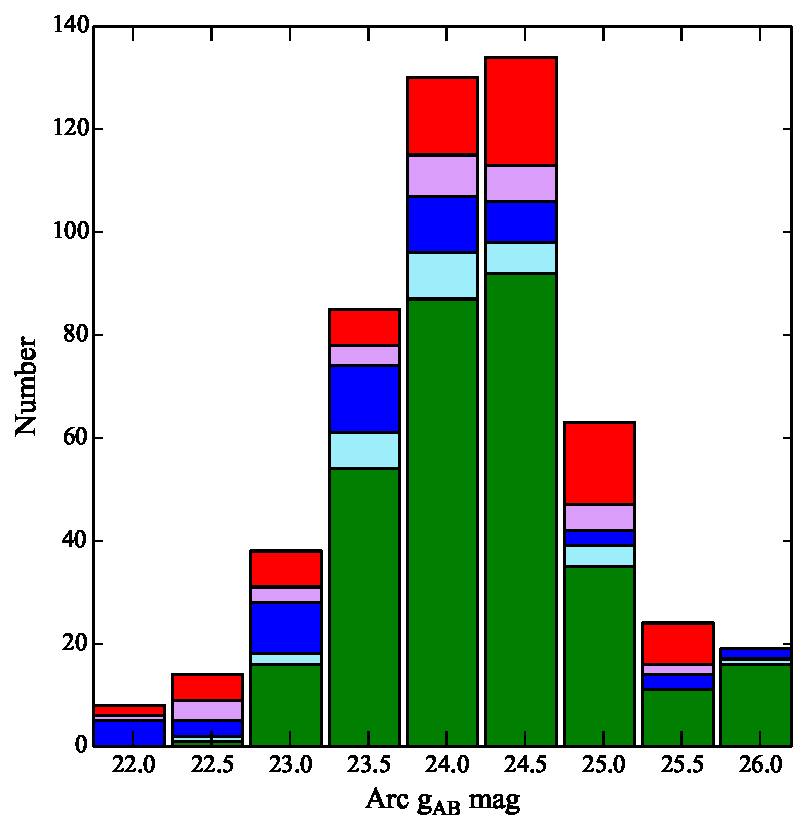
\includegraphics[scale=0.5]{sw-cfhtls-figs/stacked_lenscand_mag.pdf}
\caption{ \label{fig:stackre}
Candidate detections by the \rf, \sw and the \af as a
function of the Einstein radius and $g$ band magnitude of the lensed
images. (XXXX check how different are the estimates from the different
measurement techniques for a given lens candidates.) }
\end{center}
\end{figure*}


\begin{figure}
\begin{center}
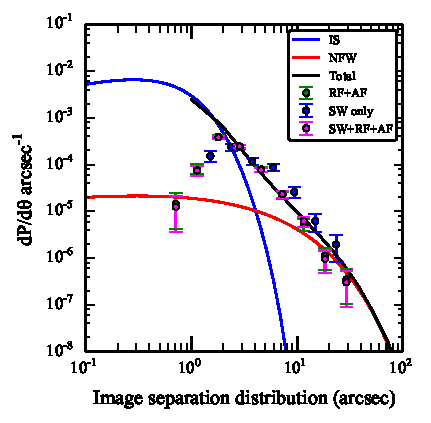
\includegraphics[scale=1.2]{sw-cfhtls-figs/isd_cfhtls_sw.pdf}
\caption{ \label{fig:isd} Image separation distribution. Comparing
theoretical predictions (solid curves) with the \cfhtls known lens
samples (REF , green points) and the same \cfhtls sample after combining
with the incremental lens sample from \sw (magenta points). The \sw only
sample including new and known lens candidates are shown with blue
points. }
\end{center}
\end{figure}


Efficiency of a visual search can vary in different sections of an
image. Our eyes tend to focus usually at the center of an image and lens
candidates close to the borders could go undetected. Therefore, it is
essential to test and understand if \sw tends to miss certain lenses
because they happen to be close to the borders of the image cutouts.
 
From the SWAP, the image cutouts inspected by the \sw volunteers receive
a status of detected (if P$>$P$_{\rm acc_thresh}$), rejected (if
P$<$P$_{\rm rej_thresh}$) and undecided (if P$_{\rm rej_thresh}$ $<$ P
$<$ P$_{\rm acc_thresh}$). In \Fref{fig:comppos}, we compare the
positions of simulated lenses which are detected (red), undecided
(green) and rejected (blue). We also make the same comparison for the
known lens candidates in the right panel.  We note that for some cases
randomly selected subsamples are shown for the ease of visual
comparison. For example, the absolute number of simulated lenses
detected is too high compared to the rejected sample. We do not find any
strong visual correlation in the rate of detections as a function of the
position for both the simulated and the known lens sample. Thus, the
completeness of the lens sample does not seem to be significantly
affected by whether a lens is located close to the border or well within
the center.

% % % % % % % % % % % % % % % % % % % % % % % % % % % % % % % % % % % % % % % 
\subsection{Why \sw candidates were missed by lens finding robots?}

The new lens candidates discovered by \sw are run through the \rf to
trace and understand at what stage the algorithm failed to detect them.

At the first step of the \rf algorithm, a galaxy catalog is generated
based on magnitude, redshift and SED type \citep[see]{Gavazzi2014} to
select galaxies which are most likely to act as lenses. We find that
about 40\% of the new \sw candidates fail to meet this initial selection
criteria e.g. SW1, SW13, SW19, SW22, SW27 and SW30.  All of the lensing
galaxies are bright enough to satisfy the $i<22$ criterion. However,
some of them have a bright companion galaxy, some of them do not look
like E/S0 type galaxies and some are edge on galaxies. {\bf there are a
few which look regular galaxies so which criteria are they failing??} 

%% 13 are under mask so no photoz, 10 have photoz (z>0.2 except for 1). 

In the following steps, the flux from the galaxy is subtracted from the
scaled difference image to enhance the visibility of the faint blue
lensed features. An object finder is run on this image to quantify the
lensed image properties. About 50\% of the \sw candidates could not be
detected by the object finder because properties such as the image area,
axis ratio, magnitude/color and alignment with respect to the lensing
galaxy are not satisfied. Some of the candidates missed at this stage
are e.g. SW4, SW5, SW6, SW26, SW36, SW39 and SW47. 

%% 23/61 miss first step, 30/61 miss auto, 5 pass auto but have poor
%grade from visual classf.

Next, we rerun the \af on the same \sw sample of new candidates. The \af
is directly run an image to look for elongated arc like objects and does
not require a list of targets to begin with. Objects are identified by
placing thresholds on the noise level in the images. Thus, \af
detections are sensitive to changes in the noise levels. Also, the size
of the PSF is important to know what dimensions should be expected for
the arc candidates.  

Originally, the \af was run on a large image with an area of $\sim 19400
\times 19400$ pixels$^2$. For the rerun, we work with much smaller
images because this is faster but this affects the number and type of
arc detections. We find that about 30\% of the new candidates are detected
without changing any of the thresholds in the code because of the change
in the noise level.

{\bf TBD: 
comment on any lensed quasars, on any exotic lenses;
of course, there must be lenses which cannot be detected currently by
either robots/humans
check if some candidates were detected because they were hidden
underneath the sims ie. from the D11;
}


% % % % % % % % % % % % % % % % % % % % % % % % % % % % % % % % % % % % % % % 
\subsection{Limitations and Caveats of the training sample}

The simulated sample is not perfect because our understanding of various
phenomena in the Universe is not complete and because of the uncertainties in
the parameters of our model. Here, we describe some of the cases or
aspects in which the simulations are known to have failed or seem
unrealistic. 

The parameters required by various scaling relations and the models primarily
depend on the photometry of the galaxies, groups and quasars detected in the
survey. For galaxy-scale lenses, the lensing galaxies at higher redshifts or
which are fainter have poor photometric measurements. This causes relatively
larger uncertainties in its luminosity and velocity dispersion and leads to
simulated lenses which look implausible. For example, due to a larger
uncertainty in the velocity dispersion of the lensing galaxy, the lensed images
may have larger image separation than what is expected given the visual priors
from the galaxy.

At group-scales, the photometric and redshift estimates are used when
defining the group membership. Therefore, errors in redshift estimates generate
galaxy groups with BGG or member galaxies with dissimilar properties. In some
cases, low redshift spiral galaxies are incorrectly assigned high redshift.
Spiral galaxies are typically less massive and low redshift spiral galaxies are
unlikely to act as gravitational lenses. Hence, the resulting simulated lenses
are not convincing.

We use single Sersic component to describe the light profiles of background
galaxies. This is clearly not the most accurate description for galaxies,
especially, star-forming galaxies which form a significant fraction of the
lensed galaxy population. Star-forming galaxies have complex structures such as
star forming knots, spiral arms, bars and disks. 

\begin{figure*}
\begin{center}
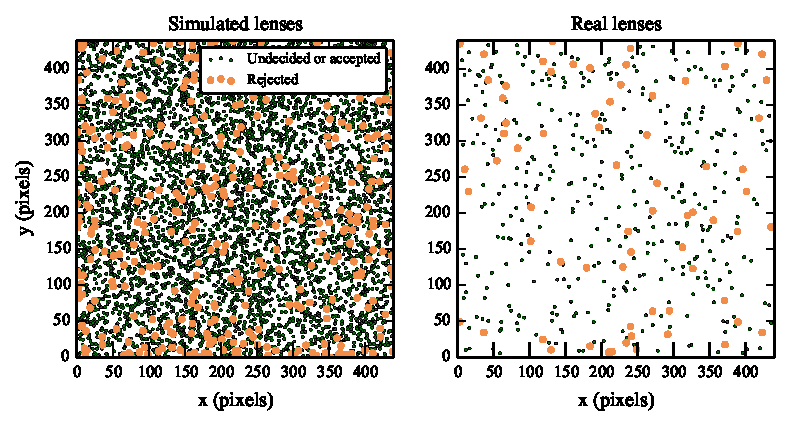
\includegraphics[scale=0.95]{sw-cfhtls-figs/completeness_pos.pdf}
\caption{ \label{fig:comppos}
Completeness as a function of position of lens systems. Simulated lenses
(left) and real lens candidates (right) are shown. Irrespective of the
status of the lenses, that is, detected, undecided or rejected, there is
no strong dependency on where the lenses are located both for the
simulated and the real sample of lens candidates. }
\end{center}
\end{figure*}

%%%%%%%%%%%%%%%%%%%%%%%%%%%%%%%%%%%%%%%%%%%%%%%%%%%%%%%%%%%%%%%%%%%%%%%%%%%%%%

\section{Summary and Conclusions}
\label{sec:conclude}
In this paper, we describe the framework and procedure used to generate
simulated lens sample for the blind lens search in the \cfhtls survey in
collaboration with \sw. The aim of this lens search is to find lenses that have
been missed by lens finding algorithms. The simulated lens sample is used for
training the citizen scientists, calibrating their performance and rejecting
unlikely lenses from the sample based on the classifications of citizen
scientists. As a result, the simulated lenses need to consist of realistic
looking lenses.

We use the photometric and redshift catalogues for the foreground galaxies and
additionally, color catalogues for background galaxies and quasars. We
use scaling relations to relate light properties to properties such as mass and
size to generate lens models. We further account for the
instrumental effects such as seeing and noise before creating the final lensed
images of model background sources. We add the lensed images on top of the real
galaxies and groups in the \cfhtls data in all filters.

We draw the following conclusions:

\begin{itemize} 

\item Crowd-sourced gravitational lens detection works, as shown in by comparing with real lenses in CFHTLS:
Real (robotically-detected and expert-confirmed) lenses are
recovered/missed at similar/comparable/different rates C’\% and P’\% - this is a partial test of supervised vs unsupervised learning

%Which real lenses were missed? False negatives

\item We found a sample of new gravitational lens candidates. An
expert-graded sample of 74 with 44 promising and 30 low probability
candiates.

The SW lenses are different from the robotically (\rf and \af) detected lenses, in the following ways.
XXXXX


\end{itemize}

\onecolumn

\begin{center}
\begin{longtable}{lrrrrrrrrrr}
\caption{ \label{tab:swcands} 
Sample of the \sw new lens candidates. }\\
\hline
SW ID & Name & RA & Dec &  $z_{\rm phot}$ & $m_i$ & $R_{\rm A}$ & G & ZooID & P & Comments  \\
  &  & (deg) & (deg) &  & (mag) &  (") &  &  & & \\ 
\hline
\endfirsthead
\hline
SW ID & Name & RA & Dec &  $z_{\rm phot}$ & $m_i$ & $R_{\rm A}$ & G & ZooID & P & Comments  \\
  &  & (deg) & (deg) &  & (mag) &  (") &  &  & & \\ 
\hline
\endhead
\hline
\multicolumn{11}{p{18cm}}{
The column Comments has two type of notes. The first is about the lens
image configuration where the symbols mean the following A: Arc, D: Double, Q:
Quad, R: Ring. The second is a comment on the type of lens assessed
visually. Note that this classification is not based on colors or spectral
analysis. The symbols are E: Elliptical, S: (face on) Spiral, G: Group-scale, D:
Edge on disk, R: Red starforming galaxy.  This galaxy falls within the masked region as per the catalog from
which the magnitudes and the redshift are extracted.  
}\\  
\endlastfoot
 SW1 & CFHTLS J022409-105807 &   36.0398 &  -10.9688 &  0.0 &  0.0 &  4.8 &  3.0 & ASW0004dv8 &  1.0  &  A,G   \\ 
 SW2 & CFHTLS J140522+574333 &  211.3426 &   57.7259 &  0.7 & 19.7 &  1.0 &  2.7 & ASW000619d &  0.7  &  A,R   \\ 
 SW3 & CFHTLS J142603+511420 &  216.5149 &   51.2390 &  0.0 &  0.0 &  4.4 &  2.7 & ASW0006mea &  0.7  &  A,G   \\ 
 SW4 & CFHTLS J142934+562541 &  217.3926 &   56.4281 &  0.5 & 19.0 &  5.9 &  2.7 & ASW0009cjs &  0.8  &  A,G   \\ 
 SW5 & CFHTLS J143454+522850 &  218.7270 &   52.4808 &  0.6 & 19.4 &  4.4 &  2.7 & ASW0007k4r &  0.4  &  Q,G/R   \\ 
 SW6 & CFHTLS J143627+563832 &  219.1164 &   56.6425 &  0.5 & 19.4 &  1.5 &  2.7 & ASW0008swn &  0.9  &  A,D   \\ 
 SW7 & CFHTLS J220256+023432 &  330.7369 &    2.5758 &  0.0 &  0.0 &  6.8 &  2.7 & ASW0007e08 &  0.8  &  A,G/C   \\ 
 SW8 & CFHTLS J020832-043315 &   32.1340 &   -4.5543 &  1.0 & 21.0 &  1.6 &  2.3 & ASW0002asp &  1.0  &  A,R   \\ 
 SW9 & CFHTLS J020848-042427 &   32.2011 &   -4.4075 &  0.8 & 20.5 &  1.1 &  2.3 & ASW0002bmc &  0.9  &  D,D   \\ 
SW10 & CFHTLS J020849-050429 &   32.2078 &   -5.0749 &  0.8 & 20.6 &  0.9 &  2.3 & ASW0002qtn &  1.0  &  A,R   \\ 
SW11 & CFHTLS J022406-062846 &   36.0256 &   -6.4796 &  0.4 & 19.6 &  0.9 &  2.3 & ASW0003wsu &  0.7  &  A,E   \\ 
SW12 & CFHTLS J022805-051733 &   37.0236 &   -5.2927 &  0.4 & 18.8 &  1.4 &  2.3 & ASW0009ans &  1.0  &  Q,E   \\ 
SW13 & CFHTLS J023123-082535 &   37.8468 &   -8.4266 &  0.0 &  0.0 &  1.2 &  2.3 & ASW0004xjk &  0.3  &  A,R   \\ 
SW14 & CFHTLS J084841-045237 &  132.1708 &   -4.8772 &  0.3 & 19.0 &  1.0 &  2.3 & ASW0004nan &  1.0  &  A,E   \\ 
SW15 & CFHTLS J140030+574437 &  210.1260 &   57.7437 &  0.4 & 18.2 &  2.0 &  2.3 & ASW0009bp2 &  0.6  &  A,E   \\ 
SW16 & CFHTLS J140622+520942 &  211.5958 &   52.1617 &  0.7 & 20.3 &  1.2 &  2.3 & ASW0005rnb &  0.7  &  A,R   \\ 
SW17 & CFHTLS J143658+533807 &  219.2425 &   53.6355 &  0.7 & 19.6 &  0.9 &  2.3 & ASW0007hu2 &  0.6  &  D,D   \\ 
SW18 & CFHTLS J020642-095157 &   31.6750 &   -9.8658 &  0.2 & 20.8 &  0.9 &  2.0 & ASW0001ld7 &  0.8  &  A,R   \\ 
SW19 & CFHTLS J021221-105251 &   33.0881 &  -10.8811 &  0.3 & 17.9 &  1.8 &  2.0 & ASW0002dx7 &  0.8  &  D,E/S   \\ 
SW20 & CFHTLS J022533-053204 &   36.3888 &   -5.5346 &  0.5 & 19.4 &  3.6 &  2.0 & ASW0004m3x &  0.4  &  A,R/G   \\ 
SW21 & CFHTLS J022716-105602 &   36.8186 &  -10.9341 &  0.4 & 17.2 &  1.8 &  2.0 & ASW0009ab8 &  0.7  &  A,E/G   \\ 
SW22 & CFHTLS J023008-054038 &   37.5359 &   -5.6774 &  0.6 & 19.7 &  1.9 &  2.0 & ASW0003r61 &  0.5  &  A,E   \\ 
SW23 & CFHTLS J023051-082423 &   37.7141 &   -8.4064 &  0.0 &  0.0 &  0.8 &  2.0 & ASW000412m &  0.4  &  A,E   \\ 
SW24 & CFHTLS J023315-042243 &   38.3133 &   -4.3789 &  0.7 & 19.7 &  1.0 &  2.0 & ASW00050sk &  0.8  &  A,R   \\ 
SW25 & CFHTLS J090308-043252 &  135.7844 &   -4.5479 &  0.0 &  0.0 &  1.2 &  2.0 & ASW00007mq &  0.6  &  A,E   \\ 
SW26 & CFHTLS J135755+571722 &  209.4827 &   57.2897 &  0.8 & 20.2 &  1.3 &  2.0 & ASW0005ma2 &  0.8  &  D,D   \\ 
SW27 & CFHTLS J141432+534004 &  213.6372 &   53.6679 &  0.7 & 21.4 &  0.9 &  2.0 & ASW0006jh5 &  0.8  &  A,R   \\ 
SW28 & CFHTLS J143055+572431 &  217.7333 &   57.4088 &  0.7 & 19.3 &  1.0 &  2.0 & ASW0007wfj &  0.9  &  A,R   \\ 
SW29 & CFHTLS J143838+572647 &  219.6589 &   57.4464 &  0.8 & 20.2 &  1.1 &  2.0 & ASW0008qsm &  0.9  &  A,R   \\ 
SW30 & CFHTLS J021057-084450 &   32.7414 &   -8.7474 &  0.0 &  0.0 &  2.5 &  1.7 & ASW0002p8y &  0.4  &  A,G   \\ 
SW31 & CFHTLS J021514-092440 &   33.8109 &   -9.4111 &  0.7 & 19.9 &  2.6 &  1.7 & ASW00021r0 &  0.4  &  A,R/G   \\ 
SW32 & CFHTLS J022359-083651 &   35.9995 &   -8.6143 &  0.0 &  0.0 &  3.1 &  1.7 & ASW0004iye &  0.4  &  A,E   \\ 
SW33 & CFHTLS J022745-062518 &   36.9387 &   -6.4218 &  0.6 & 20.5 &  1.2 &  1.7 & ASW0003s0m &  0.5  &  A,R   \\ 
SW34 & CFHTLS J023453-093032 &   38.7232 &   -9.5089 &  0.5 & 19.8 &  0.7 &  1.7 & ASW00051ld &  0.3  &  A,D   \\ 
SW35 & CFHTLS J084833-044051 &  132.1385 &   -4.6809 &  0.8 & 20.2 &  0.9 &  1.7 & ASW0004wgd &  0.7  &  A,R   \\ 
SW36 & CFHTLS J090248-010232 &  135.7020 &   -1.0424 &  0.4 & 19.1 &  1.4 &  1.7 & ASW000096t &  0.6  &  D,E   \\ 
SW37 & CFHTLS J143100+564603 &  217.7511 &   56.7675 &  0.0 &  0.0 &  1.8 &  1.7 & ASW00086xq &  0.8  &  A,E   \\ 
SW38 & CFHTLS J143353+542310 &  218.4736 &   54.3862 &  0.8 & 19.8 &  1.6 &  1.7 & ASW0009cox &  0.6  &  A,R/G   \\ 
SW39 & CFHTLS J220215+012124 &  330.5635 &    1.3567 &  0.3 & 17.4 &  4.6 &  1.7 & ASW0005qiz &  0.5  &  rA,G   \\ 
SW40 & CFHTLS J221306+014708 &  333.2758 &    1.7856 &  0.0 & 17.1 &  1.4 &  1.7 & ASW0008wmr &  0.9  &  A,S   \\ 
SW41 & CFHTLS J221513+010240 &  333.8056 &    1.0446 &  0.0 &  0.0 &  0.8 &  1.7 & ASW0008dxh &  0.3  &  A,R/G   \\ 
SW42 & CFHTLS J221519+005758 &  333.8321 &    0.9661 &  0.4 & 20.2 &  1.0 &  1.7 & ASW0008xbu &  0.8  &  A,D   \\ 
SW43 & CFHTLS J221716+015826 &  334.3189 &    1.9739 &  0.1 & 21.6 &  1.0 &  1.7 & ASW00096rm &  1.0  &  A/R,R   \\ 
SW44 & CFHTLS J020810-040220 &   32.0450 &   -4.0389 &  1.0 & 20.8 &  1.8 &  1.3 & ASW0001c3j &  0.7  &  A,R   \\ 
SW45 & CFHTLS J021021-093415 &   32.5898 &   -9.5711 &  0.4 & 18.4 &  2.7 &  1.3 & ASW0002k40 &  0.4  &  D,S   \\ 
SW46 & CFHTLS J021225-085211 &   33.1051 &   -8.8697 &  0.8 & 19.5 &  2.1 &  1.3 & ASW00024id &  1.0  &  R,R   \\ 
SW47 & CFHTLS J021317-084819 &   33.3234 &   -8.8055 &  0.5 & 19.8 &  1.3 &  1.3 & ASW00024q6 &  0.4  &  A,R/E   \\ 
SW48 & CFHTLS J022843-063316 &   37.1794 &   -6.5547 &  0.5 & 19.1 &  1.8 &  1.3 & ASW0003r6c &  0.3  &  D/A,E   \\ 
SW49 & CFHTLS J090219-053923 &  135.5794 &   -5.6566 &  0.0 &  0.0 &  2.0 &  1.3 & ASW0000g95 &  1.0  &  A,R/E   \\ 
SW40 & CFHTLS J090319-040146 &  135.8311 &   -4.0297 &  0.0 & 19.8 &  1.2 &  1.3 & ASW00007ls &  0.5  &  A,R/E   \\ 
SW51 & CFHTLS J090333-005829 &  135.8886 &   -0.9749 &  0.0 &  0.0 &  2.1 &  1.3 & ASW00008a0 &  1.0  &  A/D,E/G   \\ 
SW52 & CFHTLS J135724+561614 &  209.3536 &   56.2707 &  0.0 &  0.0 &  2.6 &  1.3 & ASW0006e0o &  0.9  &  D,E   \\ 
SW53 & CFHTLS J140027+541028 &  210.1164 &   54.1746 &  0.0 &  0.0 &  1.2 &  1.3 & ASW0006a07 &  0.6  &  Q,R/E   \\ 
SW54 & CFHTLS J140425+520506 &  211.1062 &   52.0850 &  0.4 & 18.9 &  1.4 &  1.3 & ASW0005o0w &  0.6  &  D,E   \\ 
SW55 & CFHTLS J141518+513915 &  213.8290 &   51.6542 &  0.4 & 18.3 &  3.0 &  1.3 & ASW00070vl &  0.8  &  D,E   \\ 
SW56 & CFHTLS J142620+561356 &  216.5870 &   56.2323 &  0.5 & 19.5 &  1.3 &  1.3 & ASW0007sez &  0.8  &  A/R,S   \\ 
SW57 & CFHTLS J142652+560002 &  216.7201 &   56.0006 &  0.0 &  0.0 &  1.5 &  1.3 & ASW0007t5y &  1.0  &  R,R   \\ 
SW58 & CFHTLS J142843+543713 &  217.1815 &   54.6204 &  0.4 & 19.7 &  1.3 &  1.3 & ASW0007pga &  0.6  &  D,D   \\ 
SW59 & CFHTLS J143631+571131 &  219.1315 &   57.1922 &  0.7 & 20.9 &  1.3 &  1.3 & ASW0008pag &  0.6  &  D/A,R   \\ 
SW60 & CFHTLS J143651+530705 &  219.2150 &   53.1183 &  0.6 & 19.2 &  3.1 &  1.3 & ASW0007h27 &  1.0  &  A,E/G   \\ 
SW61 & CFHTLS J143950+544606 &  219.9609 &   54.7686 &  0.0 &  0.0 &  1.7 &  1.3 & ASW00085cp &  0.4  &  A,G/R   \\ 
\end{longtable}
\end{center}


\twocolumn

%%%%%%%%%%%%%%%%%%%%%%%%%%%%%%%%%%%%%%%%%%%%%%%%%%%%%%%%%%%%%%%%%%%%%%%%
%%  ACKNOWLEDGMENTS
%%%%%%%%%%%%%%%%%%%%%%%%%%%%%%%%%%%%%%%%%%%%%%%%%%%%%%%%%%%%%%%%%%%%%%%%

\section*{Acknowledgements}
 
We thank all \Ncollaboration members of the \sw community for their
contributions to the project so far. A complete list of collaborators is
provided at \texttt{http://spacewarps.org/\#/results/CFHTLS}.

We are also grateful to Stuart Lynn, Kelly Borden, Laura Whyte, Brooke Simmons,
David Hogg, Thomas Jennings, Layne  Wright, Cecile Faure, Jonathan Coles, Stuart
Lowe and Jean-Paul Kneib for many useful conversations about citizen science and
gravitational lens detection, and to the Dark Energy Survey and Pan-STARRS strong
lensing science teams for their suggestions and encouragement.

PJM was given support by the Royal Society, in the form of a research
fellowship, and by the U.S. Department of Energy under contract number DE-AC02-76SF00515.
%
AV acknowledges support from the Leverhulme Trust in the form of a research
fellowship.
%
The work of AM and SM was supported by World Premier International Research
Center Initiative (WPI Initiative), MEXT, Japan. The work of AM was also supported in
part by National Science Foundation Grant No. PHYS-1066293 and the hospitality
of the Aspen Center for Physics.
%
% Zooniverse / Sloan Foundation.
%
% Other authors.
PJM and ES thank the Institute of Astronomy and Astrophysics, Academia Sinica
(ASIAA) and Taiwan's Ministry of Science and Technology (MOST) for their
financial support of the workshop ``Citizen Science in Astronomy'' in March
2014, at which some parts of the SWAP analysis was developed.

The \sw project is open source.
The web app was developed at \texttt{https://github.com/Zooniverse/Lens-Zoo}, and was supported by a grant from the Alfred P. Sloan Foundation, 
while the SWAP analysis software was developed at
\texttt{https://github.com/drphilmarshall/SpaceWarps}.

The CFHTLS data used in this work are based on observations obtained with
MegaPrime/MegaCam, a joint project of CFHT and CEA/IRFU, at the
Canada-France-Hawaii Telescope (CFHT) which is operated by the National Research
Council (NRC) of Canada, the Institut National des Science de l'Univers of the
Centre National de la Recherche Scientifique (CNRS) of France, and the
University of Hawaii. This work is based in part on data products produced at
Terapix available at the Canadian Astronomy Data Centre as part of the
Canada-France-Hawaii Telescope Legacy Survey, a collaborative project of NRC and
CNRS.

This work is based on observations obtained with MegaPrime/MegaCam, a joint
project of CFHT and CEA/IRFU, at the Canada-France-Hawaii Telescope (CFHT) which
is operated by the National Research Council (NRC) of Canada, the Institut
National des Sciences de l'Univers of the Centre National de la Recherche
Scientifique (CNRS) of France, and the University of Hawaii. This research used
the facilities of the Canadian Astronomy Data Centre operated by the National
Research Council of Canada with the support of the Canadian Space Agency.
CFHTLenS data processing was made possible thanks to significant computing
support from the NSERC Research Tools and Instruments grant program.

%%%%%%%%%%%%%%%%%%%%%%%%%%%%%%%%%%%%%%%%%%%%%%%%%%%%%%%%%%%%%%%%%%%%%%%%%%%%%%
%  APPENDICES
%%%%%%%%%%%%%%%%%%%%%%%%%%%%%%%%%%%%%%%%%%%%%%%%%%%%%%%%%%%%%%%%%%%%%%%%%%%%%%

\appendix


%%%%%%%%%%%%%%%%%%%%%%%%%%%%%%%%%%%%%%%%%%%%%%%%%%%%%%%%%%%%%%%%%%%%%%%%%%%%%%
%  REFERENCES
%%%%%%%%%%%%%%%%%%%%%%%%%%%%%%%%%%%%%%%%%%%%%%%%%%%%%%%%%%%%%%%%%%%%%%%%%%%%%%

% MNRAS does not use bibtex, input .bbl file instead. 
% Generate this in the makefile using bubble script in scriptutils:

% bubble -f paper-lcr.tex references.bib 
% \input{paper-lcr.bbl}

\bibliographystyle{apj}
\bibliography{references_cfhtls}
%\bibliography{references}


%%%%%%%%%%%%%%%%%%%%%%%%%%%%%%%%%%%%%%%%%%%%%%%%%%%%%%%%%%%%%%%%%%%%%%%%%%%%%%

\label{lastpage}
\bsp

\end{document}

%%%%%%%%%%%%%%%%%%%%%%%%%%%%%%%%%%%%%%%%%%%%%%%%%%%%%%%%%%%%%%%%%%%%%%%%%%%%%%
